\input{../preamble.tex}
\def\arraystretch{1}
\setlength\tabcolsep{5pt}

\SetDate[31/03/2026]

\begin{document}
\pagestyle{fancy}
\fancyhead[L]{Seconde 5}
\fancyhead[C]{\textbf{Exercices de colle}}
\fancyhead[R]{\today}

\begin{thm}\label{thm:1}
	Un point $(x ; y)$ appartient à la courbe représentative $\C_f$ d'une fonction $f$ si et seulement si
		\[ y = f(x). \]
\end{thm}

\begin{dfn}\label{def:1}
	Pour un point $A(x_A ; y_A)$, un vecteur $v=\pvec{a}{b}$, et un nombre $k\in\R$, on pose
		\[ A + kv = A + \pvec{ka}{kb} = (x_A + ka ; y_A + kb). \]
\end{dfn}

\exe{}{
	Considérons $A(0;4)$ un point et $v=\pvec2{-4}$ un vecteur.
	\begin{enumerate}
		\item
		Placer le point $A$ dans le repère ci-dessous et y représenter le vecteur $v$.
		\item
		À l'aide de la définition \ref{def:1}, calculer les coordonnées des points
			\begin{align*}
				B = A+v, && C = A+\frac12v, && D = A - v, && E = A - \frac32v.
			\end{align*}
		Par exemple, $B(2;0)$ et $E(-3 ; 10)$.
		\item
		Placer les points $B, C, D, E$ dans le repère ci-dessous.
		\item
		Montrer que $v$ et $\pvec1{-2}$ sont colinéaires en montrant que l'un est multiple de l'autre.
		\item
		Écrire l'expression algébrique de la fonction $f(x) = ax+b$ en remplaçant $a$ par $-2$ et $b$ par $4$.
		\item
		Montrer, à l'aide du théorème \ref{thm:1}, que
			\begin{align*}
				A\in\C_f, && B\in\C_f, && C\in\C_f, && D\in\C_f, && E\in\C_f.
			\end{align*} 
	\end{enumerate}
	
	\begin{center}
	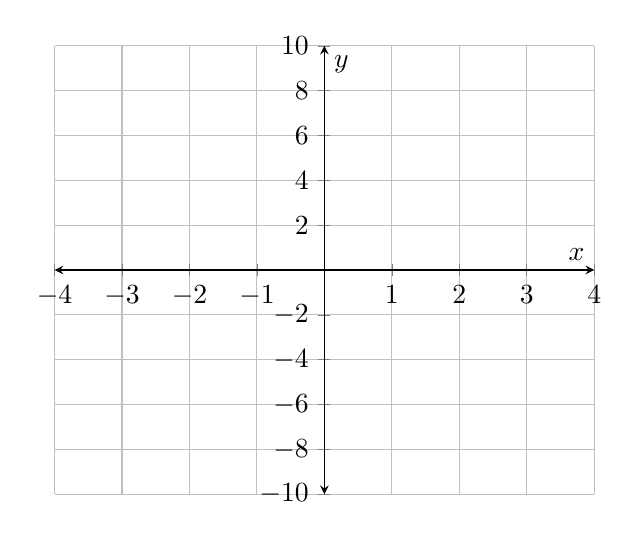
\begin{tikzpicture}[>=stealth, scale=1]
		\begin{axis}[xmin = -4, xmax=4, ymin=-10, ymax=10, axis x line=middle, axis y line=middle, axis line style=<->, xlabel={}, ylabel={}, xtick distance=1, ytick distance=2, grid=both, xlabel=$x$, ylabel=$y$]
		\end{axis}
	\end{tikzpicture}
	\end{center}
}{exe:1}{
	
}

\begin{thm}\label{thm:2}
	Soit $f(x) = ax+b$ une fonction affine.
	Alors
		\begin{align*}
			b = f(0), && \et && a = f(1) - f(0).
		\end{align*}
\end{thm}

\exe{}{
	À l'aide du théorème \ref{thm:2}, calculer le coefficient directeur $a$ et l'ordonnée à l'origine $b$ des fonctions affines suivantes.
	
	\begin{multicols}{2}
	\begin{enumerate}
		\item $f(x) = 2x+1$
		\item $g(x) = 2- \dfrac23 x $
		\item $h(x) = x$
		\item $i(x) = 2-x$
		\item $j(x) = \frac{x}2+1$
		\item $k(x) = 7$
		\item $l(x) = 0$
		\item $m(x) = -\frac{3x}{6}$
	\end{enumerate}
	\end{multicols}
}{exe:2}{
	
}

\begin{thm}
	Soient $f$ et $g$ deux fonctions sur $\R$.
	Un point $P(x_P; y_P)$ à l'intersection des deux courbes représentatives de $f$ et $g$ doit vérifier $y_P = f(x_P) = g(x_P)$.
		\begin{align*}
			(x_P ; y_P) \in \C_f \cap \C_g \iff y_P = f(x_P) = g(x_P)
		\end{align*}
\end{thm}



\begin{exemple}
	Soient $f(x) = 3x + 5$ et $g(x) = 2x + 7$ deux fonctions affines.
	Trouvons le point $(x;y)$ d'intersection de $\C_f$ et $\C_g$.
	
	D'abord, l'abscisse $x$ vérifie
		\begin{align*}
			f(x) &= g(x) \\
			3x+5 &= 2x+7 \\
			3x-2x &= 7 - 5 \\
			x &= 2
		\end{align*}
	Ensuite, l'ordonnée $y$ vérifie $y=f(x) = f(2) = 3\times2+5 = 11$.
	
	Finalement, $(2 ; 11)$ est le point d'intersection de $\C_f$ et $\C_g$
\end{exemple}

\exe{}{
	Trouver le point d'intersection des droites $\C_f$ et $\C_g$ en posant $f(x) = g(x)$ et en résolvant pour $x$, l'abscisse du point, puis en calculant l'image $f(x)$ pour obtenir l'ordonnée du point.

	\begin{multicols}{2}
	\begin{enumerate}[itemsep=10pt]
		\item $f(x) = 3x + 5$ et $g(x) = 2x + 7$
		\item $f(x) = 4x - 6 $ et $g(x) = 3x + 8$
		\item $f(x) = 5x + 10 $ et $g(x) = 2x + 4$
		\item $f(x) = -2x + 3 $ et $g(x) = 4x - 1$
		\item $f(x) = 7x - 5 $ et $g(x) = 5x + 9$
		\item $f(x) = 6x + 4 $ et $g(x) = 3x + 12$
		\item $f(x) = -3x + 2 $ et $g(x) = -5x - 4$
		\item $f(x) = 8x - 9 $ et $g(x) = 6x + 3$
		\item $f(x) = 2x + 11 $ et $g(x) = -3x + 5$
		\item $f(x) = -4x + 7 $ et $g(x) = -x + 10$
	\end{enumerate}
	\end{multicols}
}{exe:inter-affine}
{
	\begin{multicols}{2}
	\begin{enumerate}[itemsep=10pt]
		\item $3x + 5 = 2x + 7 \iff x = 2$
		\item $4x - 6 = 3x + 8 \iff x = 14$
		\item $5x + 10 = 2x + 4 \iff x = -2$
		\item $-2x + 3 = 4x - 1 \iff x = \dfrac{2}{3}$
		\item $7x - 5 = 5x + 9 \iff x = 7$
		\item $6x + 4 = 3x + 12 \iff x = \dfrac{8}{3}$
		\item $-3x + 2 = -5x - 4 \iff x = -3$
		\item $8x - 9 = 6x + 3 \iff x = 6$
		\item $2x + 11 = -3x + 5 \iff x = \dfrac{-6}{5}$
		\item $-4x + 7 = -x + 10 \iff x = -1$
	\end{enumerate}
	\end{multicols}
}

\begin{thm}\label{thm:3}
	Soit $f(x) = ax+b$ une fonction affine. 
	Alors $(0;b) \in \C_f$ et $\pvec1{a}$ dirige la droite $\C_f$.
\end{thm}

\begin{exemple}
	Soit $A(0;-3)$ et $B(3 ; 9)$ deux points.
	Trouvons la fonction affine $f(x) = ax+b$ telle que $\C_f$ passe par $A$ et par $B$.
	
	D'abord, $(0;-3) \in \C_f$, donc $b=-3$ d'après le théorème \ref{thm:3}.
	
	Ensuite, $\vec{AB} = \pvec{3-0}{9-(-3)} = \pvec{3}{12} = 3 \pvec{1}{4}$,
	donc $a = 4$.
	Il suit que $f(x) = 4x-3$.
	
	Vérification : $f(0) = -3$ et $f(3) = 12-3 = 9$, donc $A$ et $B$ appartiennent bien à $\C_f$.
\end{exemple}

\exe{}{
	Pour chaque paire de points $A, B$, donner la fonction affine $f(x) = ax+b$ telle que la droite $\C_f$ passe par les points $A$ et $B$.
	\begin{multicols}{2}
	\begin{enumerate}
	    \item $A(0; 3), B(4; 5)$
	
	    \item $A(0; -2), B(3; 4)$
	
	    \item $A(-3; -1), B(0; 2)$
	
	    \item $A(2; 7), B(0; 7)$
	
	    \item $A(0; 6), B(2; -3)$
	\end{enumerate}
	\end{multicols}
}{exe:3}{
	
}
\newpage 

\exe{}{
	Déterminer les paramètres (coefficient directeur $a$ et ordonnée à l'origine $b$) des fonctions affines $f,g,h$ dont les courbes sont représentées ci-dessous.
	Les droites $\C_f$ et $\C_h$ sont parallèles.

	\begin{center}
		\begin{tikzpicture}[>=stealth, scale=1.5]
		\begin{axis}[xmin = -10, xmax=10, ymin=-10, ymax=10, axis x line=middle, axis y line=middle, axis line style=<->, xlabel={}, ylabel={}, xtick = {-10, -8, ..., 8, 10}, ytick = {-10, -8, ..., 8, 10}, grid=both, clip=true]
		
			\addplot[RED_E, thick, domain =-9:9, samples=2] {-x/2 + 2}  node[below=6pt] {$\mathcal{C}_f$};
			\addplot[RED_E, thick, dotted, domain =-10:-9, samples=2] {-x/2 + 2} ;
			\addplot[RED_E, thick, dotted, domain =9:10, samples=2] {-x/2 + 2};
		
		
			\addplot[olive, thick, domain =-5:7, samples=2] {3*x/2-2}  node[pos=.2, left=5pt] {$\mathcal{C}_g$};
			\addplot[olive, thick, dotted, domain =-6:-5, samples=2] {3*x/2-2} ;
			\addplot[olive, thick, dotted, domain =7:8, samples=2] {3*x/2-2};
		
		
			\addplot[black, thick, domain =-3:9, samples=2] {-x/2 + 8}  node[above=1pt, pos=.35] {$\mathcal{C}_h$};
			\addplot[black, thick, dotted, domain =-4:-3, samples=2] {-x/2 + 8} ;
			\addplot[black, thick, dotted, domain =9:10, samples=2] {-x/2 + 8};
		
			
		\end{axis}
	\end{tikzpicture}
	\end{center}
	
	
}{exe:4}{

	\begin{align*}
		f(x) &= -\dfrac12 x + 2 \\
		g(x) &= \dfrac32 x - 2 \\
		h(x) &= -\dfrac12 x + 8
	\end{align*}

}


\exe{}{
	Considérons une fonction affine $f$ telle que les points $(2;1)$ et $(-1 ; -3)$ appartiennent à $\C_f$.
	\begin{enumerate}
		\item Esquisser $\C_f$ sur $[-3; 3]$.
		\item Estimer \emph{graphiquement} à l'aide de $\C_f$ la valeur de l'ordonnée à l'origine de $f$.
	\end{enumerate}
}{exe:5}{
	
}


%%%%%%%%%%%

\newpage
\fancyhead[C]{\textbf{Solutions}}
\fancyfoot[C]{\thepage}
\shipoutAnswer

\end{document}
